%%%%%%%%%%%%%%%%%%%%%%%%%%%%%%%%%%%%%%%%%%%%%%%%%%%%%%%%%%%%%%%%%%%%%%
% LaTeX Example: Project Report
%
% Source: http://www.howtotex.com
%
% Feel free to distribute this example, but please keep the referral
% to howtotex.com
% Date: March 2011 
% 
%%%%%%%%%%%%%%%%%%%%%%%%%%%%%%%%%%%%%%%%%%%%%%%%%%%%%%%%%%%%%%%%%%%%%%
% How to use writeLaTeX: 
%
% You edit the source code here on the left, and the preview on the
% right shows you the result within a few seconds.
%
% Bookmark this page and share the URL with your co-authors. They can
% edit at the same time!
%
% You can upload figures, bibliographies, custom classes and
% styles using the files menu.
%
% If you're new to LaTeX, the wikibook is a great place to start:
% http://en.wikibooks.org/wiki/LaTeX
%
%%%%%%%%%%%%%%%%%%%%%%%%%%%%%%%%%%%%%%%%%%%%%%%%%%%%%%%%%%%%%%%%%%%%%%
% Edit the title below to update the display in My Documents
%\title{Project Report}
%
%%% Preamble
%\documentclass[paper=a4, fontsize=12pt]{report} %{scrartcl}
\documentclass[12pt, a4paper, oneside]{article}

\setlength{\parskip}{1ex plus 0.5ex minus 0.2ex}
\renewcommand{\baselinestretch}{1.1}
\usepackage[x11names,table]{xcolor}
\usepackage{float}
\usepackage[T1]{fontenc}
\usepackage{libertine} % you can choose your own font
\usepackage[english]{babel}				% English language/hyphenation
\usepackage[protrusion=true,expansion=true]{microtype}	
\usepackage{amsmath,amsfonts} % Math packages
\usepackage[pdftex]{graphicx}	
\usepackage{url}
\usepackage{verbatim} 
\usepackage{hyperref}
\hypersetup{colorlinks = true, allcolors=black}
\usepackage{cite}
\usepackage{mathtools}
\usepackage[colorinlistoftodos]{todonotes}
\usepackage[T1]{fontenc}
\usepackage{bookmark}
\usepackage{caption}
\usepackage{float}
\usepackage{enumitem}
\usepackage{textcomp}
\usepackage[sort,nameinlink]{cleveref}
\usepackage{amssymb}
\usepackage{xcolor}
\usepackage{booktabs}
\usepackage{multirow}
\usepackage{listings}
\usepackage{subcaption}
\usepackage{adjustbox}
\usepackage{algorithm}
\usepackage{algpseudocode}
\usepackage{lipsum}
\usepackage[utf8]{inputenc}
\usepackage[TS1,T1]{fontenc}
\usepackage{fourier, heuristica}
\usepackage{array, booktabs}

\usepackage{geometry}
\geometry{
	a4paper,
	total={170mm,257mm},
	left=25mm,
	right=20mm,
	top=30mm,
	bottom=30mm
}

%%% Custom sectioning
\usepackage{sectsty}
%\allsectionsfont{\normalfont\scshape}
%\allsectionsfont{\centering \normalfont\scshape}


%%% Custom headers/footers (fancyhdr package)
\usepackage{fancyhdr}
\pagestyle{fancyplain}
\fancyhead{}											% No page header
\fancyfoot[L]{}											% Empty 
\fancyfoot[C]{}											% Empty
\fancyfoot[R]{\thepage}									% Pagenumbering
\renewcommand{\headrulewidth}{0pt}			% Remove header underlines
\renewcommand{\footrulewidth}{0pt}				% Remove footer underlines
\setlength{\headheight}{13.6pt}

\lstset{breaklines}

%%%% Equation and float numbering
%\numberwithin{equation}{section}		% Equationnumbering: section.eq#
%\numberwithin{figure}{section}			% Figurenumbering: section.fig#
%\numberwithin{table}{section}				% Tablenumbering: section.tab#
\definecolor{MyDarkGreen}{rgb}{0.0,0.4,0.0}

\lstset{ % Use Perl in this example
	frame=single, % Single frame around code
	basicstyle=\small\ttfamily, % Use small true type font underlined and blue
	identifierstyle=, % Nothing special about identifiers                                         
	showstringspaces=false, % Don't put marks in string spaces
	tabsize=3, % 5 spaces per tab
	%
	% Put standard Perl functions not included in the default language here
	morekeywords={rand},
	%
	% Put Perl function parameters here
	morekeywords=[2]{on, off, interp},
	%
	% Put user defined functions here
	%	morekeywords=[3]{test},
	%
	numbers=left, % Line numbers on left
	firstnumber=1, % Line numbers start with line 1
	stepnumber=5 % Line numbers go in steps of 5
}

%%% Maketitle metadata
\newcommand{\horrule}[1]{\rule{\linewidth}{#1}} 	% Horizontal rule

\title{
	\pagestyle{empty}
	%\vspace{-1in} 	
	\usefont{OT1}{bch}{b}{n}
	\normalfont \normalsize \textsc{Ho Chi Minh City University of Technology\\Faculty of Computer Science and Engineering}\\ [48pt]
	{\large -- CO2019 Computer Hardware -- Spring 2019 -- }
	\horrule{0.5pt} \\[0.4cm]
	\huge User Manual for the System
	\horrule{2pt} \\[0.5cm]
}
\author{
	Ho Le Thuc Quyen - 1752454\\
	Truong Le Vinh Khoa - 1752298\\
}
\date{\today}



%%% Begin document
\begin{document}
\begin{titlepage}
	\maketitle
	\thispagestyle{empty}
\end{titlepage}

\newpage
%\clearpage
%\thispagestyle{empty}
\pagenumbering{roman}
\tableofcontents

\newpage
\listoffigures
\newpage

%\newpage
%\listoftables

\newpage
\pagenumbering{arabic}
\setcounter{page}{1}

%\maketitle
\suppressfloats %No figures on first page

\section{Introduction}

The demonstration of a system with node MCU processor, RFID card reader, SIM 800 and DHT sensor. (picture top and bottom)
The system allows user to read the temperature and humidity and send the data to server if wifi is connected, otherwise, it will send to SMS.\\

\section{Overall properties of the circuit}

\subsection{Function}
Out circuit can execute the following functions:
\begin{enumerate}
	\item Access the system.
	\item Send the message to server or another mobile phones.
	\item Detect the current temperature and humid.
	\item Access WiFi.
	\item Access Server.
	\item Add more users.
\end{enumerate}
\subsection{Components}
\begin{itemize}
	\item NodeMCU:\quad
	Used as the main interface for all the connection.
	\begin{figure}[H]
		\centering
		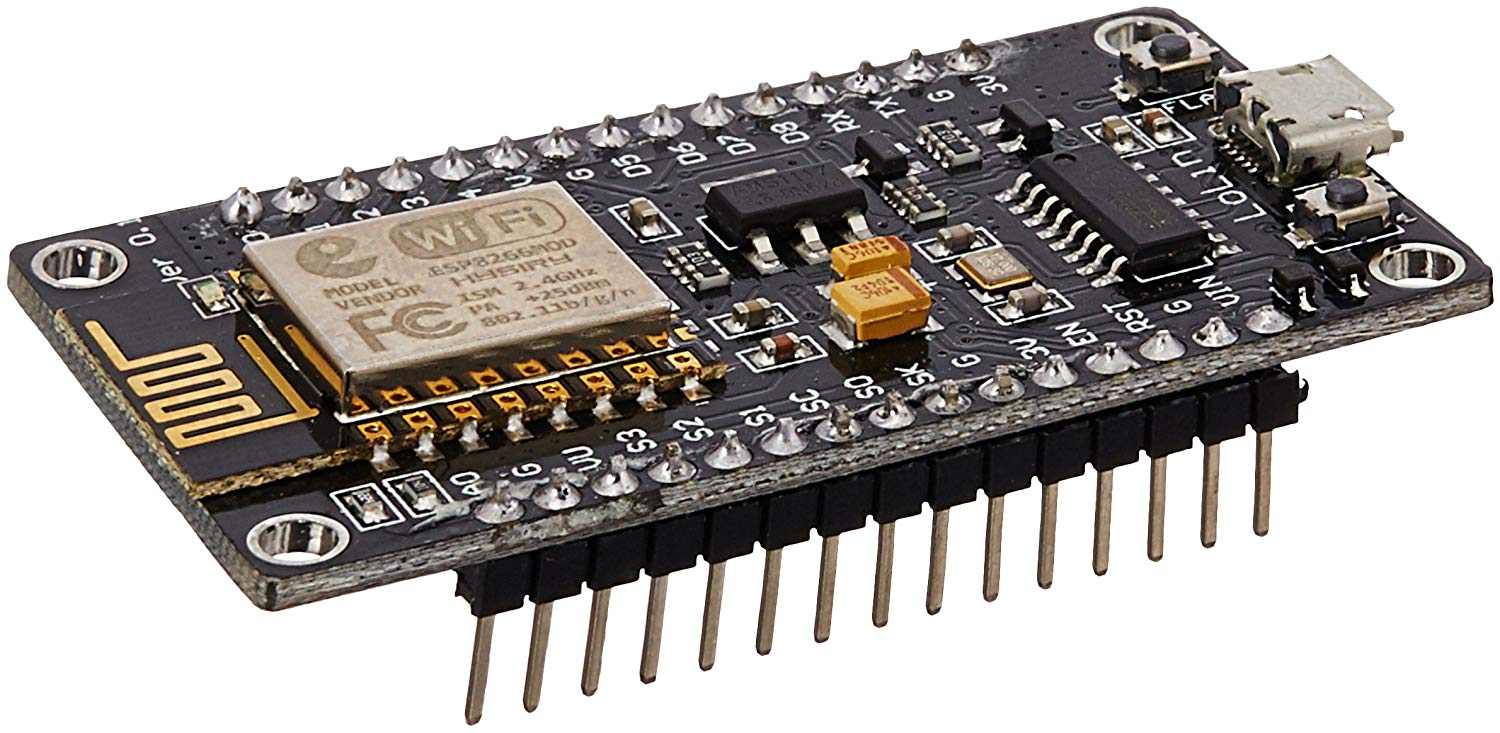
\includegraphics[width=0.4\linewidth]{nodeMCu}
		\caption{NodeMCU}
		\label{fig:ModelSim and De2i-150 board}
	\end{figure}
	\item RFID: \quad 
	Read the UID of card master card in order to access the application or used to read and add more card-users.
	\begin{figure}[H]
		\centering
		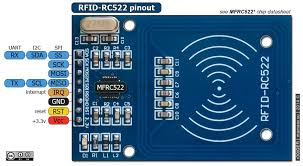
\includegraphics[width=0.4\linewidth]{RFID}
		\caption{RFID RC522}
		\label{fig:ModelSim and De2i-150 board}
	\end{figure}
	\item LCD:\quad 
	Display the content.
	\begin{figure}[H]
		\centering
		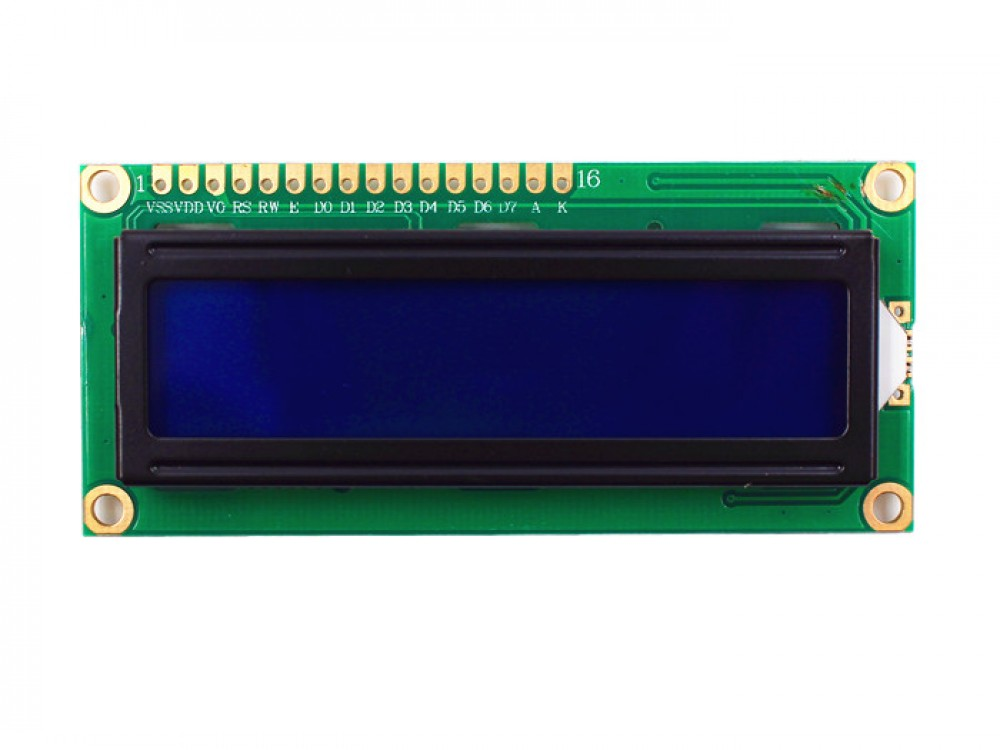
\includegraphics[width=0.4\linewidth]{LCD}
		\caption{LCD}
		\label{fig:ModelSim and De2i-150 board}
	\end{figure}
	\item SIM800L:\quad
	Send the massage.
	\begin{figure}[H]
		\centering
		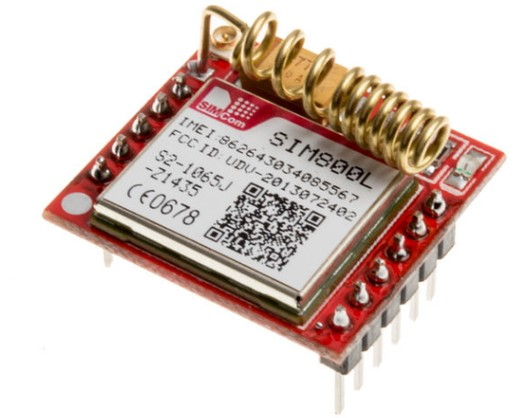
\includegraphics[width=0.3\linewidth]{SIM}
		\caption{SIM800L}
		\label{fig:ModelSim and De2i-150 board}
	\end{figure}
	\item DHT11:\quad
	Detect temperature and humid.
	\begin{figure}[H]
		\centering
		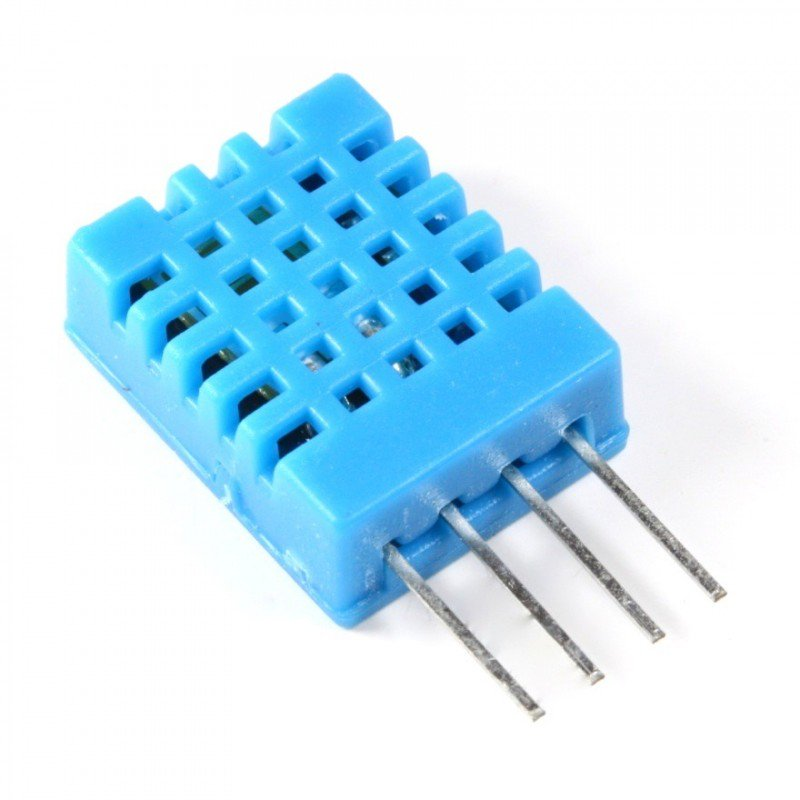
\includegraphics[width=0.35\linewidth]{DHT}
		\caption{DHT11}
		\label{fig:ModelSim and De2i-150 board}
	\end{figure}
	\item LM2596:\quad
	Used to reduce the 12V Input Voltage to 4.6V Output Voltage to raise the circuit.
	\begin{figure}[H]
		\centering
		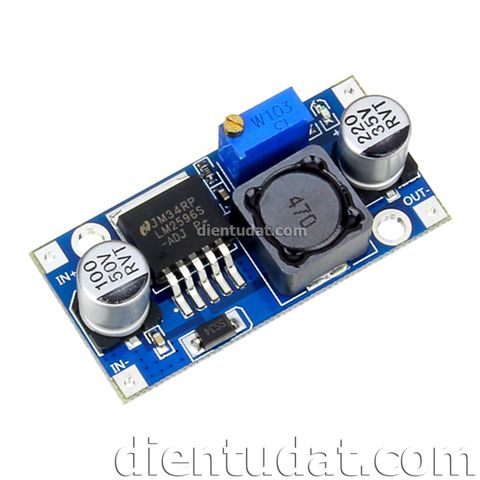
\includegraphics[width=0.4\linewidth]{LM2569}
		\caption{LM2596}
		\label{fig:ModelSim and De2i-150 board}
	\end{figure}
	\item Button: \quad Used to change between functions and select it.
	 \begin{figure}[H]
	 	\centering
	 	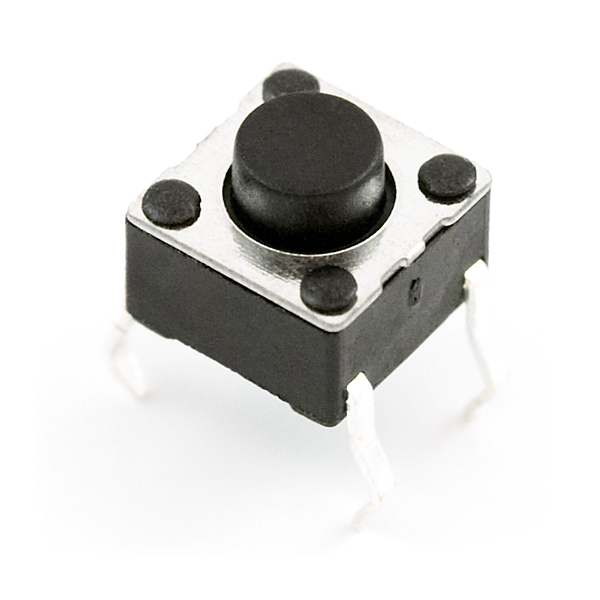
\includegraphics[width=0.3\linewidth]{button.jpg}
	 	\caption{Button}
	 	\label{fig:ModelSim and De2i-150 board}
	 \end{figure}
	  
\end{itemize}

\clearpage
\section{Instruction}
\subsection{How to control and move between tasks.  }
In this system, we mainly use two buttons to both move and control all of the functions (pointer button and choose button).\\
\\
The function of the first button (in the left side, next to LCD screen) is used as the pointer helping users to travel between the particular tasks they want.\\
\\
And the rest button (in the right side), it helps us to select the functions we want to execute.    
\subsection{Access the system}
In order to access this system, we have two ways. By master card or by additional users. \\
\\
First of all, the card member will be asked for permission to the system. If it is a right card, the system will be accessed.
A menu will be appeared to let user know what they can do, send message, see temperature and humidity, connect to wifi, connect to server, control users and quit.
\subsection{Send message}
Once users has entered to this function, a list of messages that can be sent is showed on the screen, "Hello", "What r u doing", "Eaten rice yet", "Temperature" and "Humid". When wifi is connected, the message will be sent to the server, otherwise it will be sent to mobile phone by SMS. The left button is used to select the content of message, which users want to send, and the other is pressed to send that content. If users want to quit, they can go to the line "Quit message" and go out to the main menu.

\subsection{Detect the current temperature and humid}
This task let users know the current temperature and humidity, which are displayed on the LCD screen.
\subsection{Access Wifi}
In order to access the WiFi. First, we have to declare the WiFi ID and Password in the code "PCMT.ino" at line 14 and 15. Then, after entering the system successfully, we move the pointer to the task Access Wifi and press choose button to access wifi. \\
\begin{figure}[H]
	\centering
	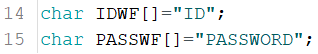
\includegraphics[width=0.6\linewidth]{wifi}
	\caption{Connecting to Wifi}
	\label{fig:ModelSim and De2i-150 board}
\end{figure}
In this process, we should not press choose button since it is processing.\\
\\
And there are two results for this task.\\
\begin{itemize}
	\item The screen will return the massage "Successfully to connect Wifi. it means that we have connected to the WiFi.
	\item  Otherwise, the screen will return "fail to connect Wifi" after 10 seconds. it means that we have typed wrong password, Id or even the connection is too weak for the system to connect.   
\end{itemize}  
\subsection{Access Sever}
Connecting to server is similar to connect Wifi. Initially, we have to declare user, password and name of your instance in CloudMQTT in file "access\_MQTT.h".
 \begin{figure}[H]
 	\centering
 	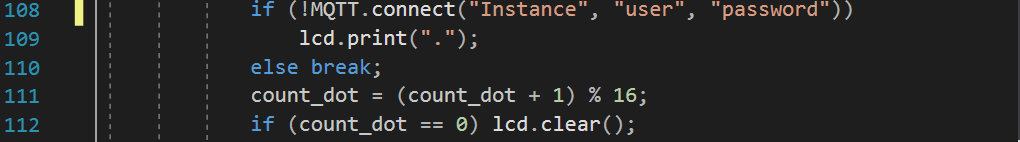
\includegraphics[width=0.8\linewidth]{server}
 	\caption{Connecting server}
 	\label{fig:ModelSim and De2i-150 board}
 \end{figure}
After pressing the choose button at access MQTT, it will return two results. Success to connect or fail to connect. If it is connected to server, i will return the result on screen simultaneously, otherwise, after 10 second, it will return fail message. 
\subsection{Control Users}
Firstly, users will be asked for insert the master card since this action is only done by master. Once the master card has inserted, the screen will display 5 users can be added to the system. The "Check users" task will find whereas the card user is added or not, if yes, it will show which user of the card is. \\
A particular user shows "EMPTY" meaning that there is no user in that slot and it can be added. The message "ADD SUCCESSFULLY" demonstrates that the card is successfully added to the system. If the card is added and the message "EXISTED CARD MEMBER - CAN NOT ADD" is shown, it shows that card has already existed in other users. \\
In contrast, the ID number, which is randomly generated for each user, is on the screen at one user if it has added before. When users insert the right user card, it will be deleted and the message will be shown, otherwise, the screen will display "NOT THE SAME CARD MEMBER". \\

	
\end{document}